\section{Parrot 2.0}
The Parrot AR.Drone is a radio controlled flying quadrotor helicopter built by the French company Parrot. The drone is designed to be
controlled by any electronic device having wi-fi connection and sufficient ressource to run a control software. Only  android, iOS and windows have offically distributed control applications. In other hand, only Windows and Linux OS are supported as a development platform.
The choice of the department for this drone as a base for the project is due to the harmless character of this quadrotor.
Two versions of the Parrot AR.Drone exists. For our project only the new version(Ar.Drone 2.0) is supported.
\subsection{Ressources}
Many ressources could be found on this UAV and this what make it one of the best choices:
\begin{itemize}
\item \url{http://www.parrot.com/fr}
%\href{http://www.parrot.com/fr}{Parrot Official Website}
\item \url{http://ardrone.parrot.com/parrot-ar-drone/usa/}
%\href{http://ardrone.parrot.com/parrot-ar-drone/usa/}{Parrot Ardrone Commercial Website}
\item \url{http://projects.ardrone.org/}
%\href{http://projects.ardrone.org/}{Ardrone Project Website}
\item \url{http://devzone.parrot.com/}
%\href{http://devzone.parrot.com/}{Parrot Developpers Website}
\end{itemize}
\subsection{Specification}
Here a quick overview of the general specification of the drone:
\begin{itemize}
\item[-] Autonomy : Approximately 12 minutes, recharging time of 1h30.
\item[-] Maximum range : 50m average, 100m in a wide-open space with few Wi-Fi waves.
\item[-] Maximum altitude : 6m is the stability limitation, 50m the wi-fi limitation (which could be hacked with wi-fi booster to go up to 75m).
\item[-] Maximum additional supported weight : ~80g is the limit of stability, ~100g is the limit of motors propulsion.
\item[-] Maximum speed : 18 km/h.
\item[-] Maximum supported wind speed : 2km/h.

\end{itemize}

\subsection{Hardware}
The hardware reference is as follow:
\begin{itemize}
\item[*] AR.Drone 1.0 : carte Mykonos, processeur ARM926EJ-S rev 5 (v5l) Wi-Fi: AR6000 Memory: 128MB RAM
\item[*] AR.Drone 2.0 : Mykonos2 card, Processor OMAP 3640 1GHz 32 bit ARM Cortex A8 with a video DSP 800MHz TMS320DMC64x
\end{itemize}

\subsection{Software}
The board has an embedded Linux with these reference : //
\begin{itemize}
\item[*] Linux myhost 2.6.27.47-parrot-01227-g93dde09 \#1 preempt Fri Jul 2 15:23:06 CEST 2010 armv5tejl GNU/Linux 
\item[*] Linux 2.6.32 kernel: Linux uclibc 2.6.32.9-g0d605ac \#1 preempt Fri Apr 6 12:01:59 CEST 2012 armv7l GNU/Linux 
\end{itemize}
This embedded linux contains these basic packages :
\begin{itemize}
\item[-] BusyBox
\item[-] Mtdutils
\item[-] zlib
\item[-] ethtool
\item[-] propcps
\item[-] udev
\item[-] dsp bridge 
\item[-] lcml dsp codec
\item[-] wireless tools
\item[-] exif
\item[-] iptables
\item[-] usbmodeswitch
\item[-] lsusb
\item[-] alsa lib
\item[-] barry
\item[-] busydroid
\item[-] webkit
\end{itemize}

We added multiple modules in order to be able to communicate with usb port:
\begin{itemize}
\item[-] cdc-acm 
\item[-] usbserial
\item[-] ftdi\_sio
\end{itemize}

you need to cross-compile these modules you can use the following step :
\begin{enumerate}
\item Download an ARM Cross-compiler you can find one on the website of Mentor Graphics (successor of Code sourcery) 
\url{http://www.mentor.com/embedded-software/sourcery-tools/sourcery-codebench/editions/lite-edition/arm-gnu-linux}
\item Install the cross-compiler :

\begin{lstlisting}
#: chmod +x arm-2012.03-57-arm-none-linux-gnueabi.bin
#: ./arm-2012.03-57-arm-none-linux-gnueabi.bin
\end{lstlisting}
\item Compile the module :
\begin{lstlisting}
#: /opt/CodeSourcery/Sourcery_CodeBench_Lite_for_ARM_GNU_Linux/bin/arm-none-linux-gnueabi-gcc -march=armv7-a toto.c -o toto.elf
\end{lstlisting}

\end{enumerate}

\subsection{Development}

\section{Arduino}

We have used the arduino board uno, without any shield or add ons. The electrical schematics is just below.\\

\begin{figure}[!h] 
\begin{center}
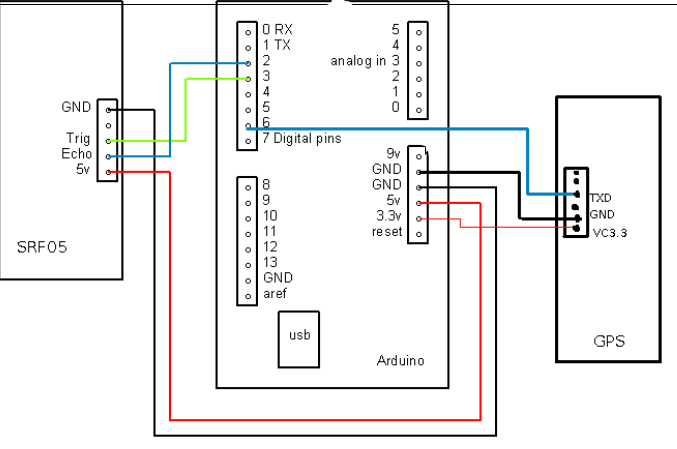
\includegraphics[width=10cm]{imgs/Capture-1.png}
\caption{Arduino schematics} 
\label{img1} 
\end{center}
\end{figure} 

Then, to upload a specific code into the board, the arduino application is needed. We used the 1.0.1 version of the application.\\

The code uploaded is :\\

\begin{lstlisting}
#include <SoftwareSerial.h>

// GPS PINS
#define SoftrxPin 2
#define SofttxPin 7
// SRF PINS
#define ECHOPIN1 3                            // Pin to receive echo pulse
#define TRIGPIN1 4                             // Pin to send trigger pulse
#define ECHOPIN2 5                            // Pin to receive echo pulse
#define TRIGPIN2 6                             // Pin to send trigger pulse
  
// initialisation de la liasion serie
SoftwareSerial gps = SoftwareSerial(SoftrxPin, SofttxPin);

int incomingByte = 0;		// Pour stocker les donnees entrantes
// Stocke la chaine GPS
char line[300] = "";
// Position dans la chaine
int index = 0;
// La chaine recherchee
char commandeGPR[7] = "$GPRMC";
// Chaine ok
int commande_ok = 0;

int i,j = 0;

int readExtractGpsGPRMC(){
// Envoie des donnees que quand on en recoit
  int ret = 0;
  
  while (gps.available () > 0)
    {
      // On lit le byte:
      incomingByte = gps.read ();
      line[index] = incomingByte;

      if (incomingByte == 10)
	{

	  // Verifie si la chaine est bien de type $GPR
	  for (int i = 0; i < 4; i++)
	    {
	      if (line[i] != commandeGPR[i])
		{
		  commande_ok = 1;
		  break;
		}
	    }
	  //-----------------------------------------------

	  // Si on a recupere la bonne chaine, on l'affiche
	  if (commande_ok == 0)
	    {
	      for (int pc = 0; pc <= index; pc++)
		{
		  Serial.write (line[pc]);
		}
             ret = 1;
	    }
	  //-------------------------------------------------
	  index = 0;
	  commande_ok = 0;
	}
      else
	{
	  index++;
	}
    }
  return ret;
}


float calculateDistance(int pinEcho, int pinTrig){
  digitalWrite(pinTrig, LOW);            // Set the trigger pin to low for 2uS
  delayMicroseconds(2);
  digitalWrite(pinTrig, HIGH);          // Send a 10uS high to trigger ranging
  delayMicroseconds(10);
  digitalWrite(pinTrig, LOW);           // Send pin low again
  
  int distance = pulseIn(pinEcho, HIGH); // Read in times pulse
  return distance/58.0;                  // Calculate distance from time of pulse                    
}

 
void setup(){
  Serial.begin(9600);// ouvre le port serie et regle le debit a 9600 bps
  gps.begin(9600);// pareil pour les ports digitaux
  pinMode(ECHOPIN1, INPUT);
  pinMode(TRIGPIN1, OUTPUT);
}

void loop(){
  unsigned long time; 
  int r = readExtractGpsGPRMC();
     
   while(r == 0) {
     r = readExtractGpsGPRMC();
   }
   time = millis();
   gps.flush();
   
   while ((millis() - time) < 600) {  
     Serial.print("$SRFR,");
     Serial.println(calculateDistance(ECHOPIN1,TRIGPIN1));
   }
}

\end{lstlisting}

Basically, in the main loop, we are extracting GPS strings and srf datas.\\

About GPS data, we just have to extract the GPRMC string of the 6 lines we receive every second.
We need to test the beginning of the string. If is equal to "\$GPRMC" string, we store the string and send it via 
serial connection to the UAV.\\

To catch SRF data, it is necessary to read the datasheet, and do the following tasks :\\

\begin{enumerate}
\item Set the trigger pin to low for 2uS
\item Send a 10uS high to trigger ranging
\item Read the time at high level, it corresponds to the duration of ultrasonic roundtrip.
\item Dividing this duration by 58, we obtain the distance to obstacle
\end{enumerate}

We have to send this distance to the UAV, like for the GPS strings.\\

Using separately ultrasonic sensors and GPS works perfectly well. However it is difficult to use both components at the same time. The GPS extraction is using SoftwareSerial class and all incoming data are stored in a buffer of this class. Data's are written every 1 second, and if we are listening this buffer all the time (except for extraction), this buffer won't overflow. But, if data are written in this buffer while we are capturing ultrasonic wave, the writting will overflow the buffer and cause the loss of some information.\\

It is impossible to multithread this program, so we have to schedule manually the execution of GPS and sensor listening. We know GPS data are incoming every second, and the execution of gps extraction last 100 ms, so we dedicate 600 ms to ultrasonic listening, and then we wait for GPS data to arrive.\\

This solution is not very satisfying because we take a margin of 300ms, and we don't have SRF data during 400ms, but we didn't find a better way to combine GPS and SRF sensors.\\

\section{Android}

\section{Ultrasonic Sensor}

\section{Bluetooth}

This part explains how to connect and read data from an android smartphone that sends information via bluetooth. ShareGPS, an application running on the phone is sending its GPS coordinate to the computer. The aim of the document is to give the process to get this coordinate.\\

First step: with the smartphone\\

\begin{itemize}
 \item Turn on the bluetooth and the GPS
 \item Launch ShareGPS and share coordinate via bluetooth
 \item Make the bluetooth visible by other devices
\end{itemize}

Second step: with the computer on Linux\\

\begin{itemize}
   \item  Turn on the bluetooth and open a terminal (you may need to be root)
   Scan devices with: ``hcitool scan''
   -> Write down the MAC address of the corresponding device
   \item Find the good channel which gives GPS coordinate with: ``sdptool records MAC\_ADDR''
   -> This command displays all channels and their functions
   -> Look for the one called ``ShareGPS'' and write down the corresponding channel
   \item Create the connection with: ``rfcomm bind X MAC\_ADDR CH''
    -> X: positive integer corresponding to the rfcomm you want to bind
    -> MAC\_ADDR: MAC address of the smartphone
    -> CH: channel of the ShareGPS application
\end{itemize}

You can now check that /dev/rfcommX exists. The last step is to read data.
To kill it use the command ``rfcomm release rfcommX'' or ``rfcomm release all''.\\

Third step: read data\\
\begin{itemize}
  \item Using PuTTY: connect via serial to /dev/rfcommX with a 9600 baudrate
  \item You can also use a self-made program
\end{itemize}

Source: \url{http://www.thinkwiki.org/wiki/How_to_setup_Bluetooth}
